\documentclass[12pt]{article}                                            
\usepackage {epsfig}
\textwidth  16.0cm
\textheight 21.5cm
\topmargin -1.0 cm
\oddsidemargin 0.5cm
\evensidemargin 0.5cm
\pagestyle{plain}
\headheight 0.3cm 
\usepackage[dvipsnames]{color} 

%%%%%%%%%%%%%%%%%%%%%%%%%%%%%%%%%%%%%%%%%%%%%%%%
\begin{document}
%%%%%%%%%%%%%%%%%%%%%%%%%%%%%%%%%%%%%%%%%%%%%%%%
\definecolor{Myred}{named}{Red}
\pagestyle{plain}
\begin{titlepage}
\begin{flushright}
~~~~~~~~~~~~~~~~~~~~~~~~~~~~~~~~~~~~~~~~~~~~~~~~~~~~~
~~~~~~~~~~~~~~~~~~~~~~~~~~~~~~~~~~~~~~~~~~~~~~~~~~~{\today}
\end{flushright}
\vskip 3.cm
\centerline{\bf \color{Myred}{M. Wood (chair), S. Manly, and A. Kim} }
\vskip 0.5cm
\centerline{\bf \LARGE \color{Myred}{Analysis Review of the :} }
\vskip 1.cm
\centerline{\bf \Large ``Study of the Hadronization}
\vskip 0.5cm
\centerline{\bf \Large of Charged Pions”''}
\vskip 0.5cm
\centerline {\bf  by R. Dupre et al.}
\vskip .5cm
%%%%%%%%%%%%%%%%%%%%%%%%%%%%%%%%%%%%%%%%%%%%%%%%%%%%%%%%%%%%%%%%%%
\end{titlepage}
\setcounter{page}{2}

The committee has reviewed the analysis note and has a number of comments that should be 
addressed.  It has been a long time since the data were taken, and it is an interesting study, so 
we encourage the authors to move forward with the improvements in order to bring it to 
publication.

{\it We would like to thank you for the thorough review and hope you will be satisfied with
our answers.} \\

This report is organized in 3 sections: lager issues to resolve, questions from the reviewers, and 
typographical corrections.  There may be some repetition between the 3 sections.  The notation 
is P\# for page \#.

{\it The answers from the authors of the note are all presented in italic script 
to allow a clear distinction.} \\

\section{Larger Issues }
1.
Ownership of the pi+ channel.  This was brought up in an email from the committee chair 
(M. Wood).  Before this analysis can move on to round 2 of the review, the ownership issue 
has to be resolved.  The NPWG chair (also M. Wood) has left it up to the eg2 group to 
resolve it.

{\it We are aware of this issue and we started regular meetings between the different 
groups toward the objective of publishing as soon as possible results coherent with
the different analysis performed on this topic (all three pions in particular). This
will eventually translate into an addendum to this note with comparisons between Hayk's 
and this analysis, which will be used to confirm the proper sizing of the systematic errors. 
In a later stage an extra analysis note from Hayk will be submitted
for the extraction of multi-dimensional results on $\pi^+$.} \\


2.
The particle ID and cuts seem to be well understood.  The acceptance correction and 
radiative corrections need to be developed. There is confusion about how the acceptance 
corrections were done (see Section 2 below). The radiative corrections are incomplete as 
reported in the note.  Both corrections need to be well-understood before the committee can 
approve of the analysis.

{\it The text about acceptance has been reviewed in details to be clearer in this new 
version. The section about radiative corrections has been updated with the new method.
We can have a meeting to clarify some of the simpler issues more rapidly.} \\

3.
In the next version, line numbers need to be added to the document for easier reference.

{\it Done.} \\

\section{Reviewers’ Questions/Comments}
1.
P3, para 2- The discussion about the importance of this to neutrino experiments misses the 
main point.  In neutrino experiments, it is true that nuclei other than hydrogen are used to 
increase the event rate and to avoid explosions.  That means that nuclear effects come into 
play.  Fermi motion and final state interactions and correlations cause confusion in the 
extraction of the signal and reconstruction of the energy of the incoming neutrino.  This 
leads to less precise determination of the oscillation parameters.  The modeling of nuclear 
effects is necessary to understand and correct for these effects.  Pion production 
measurements like this provide ways to tune the models and look at the A dependence.  The 
A dependence is very important in part because in the long baseline experiments sometimes 
the near detector and far detectors are made of different materials.  In DUNE, for example, 
the far detector will be a liquid argon TPC.  It is not yet clear that a liquid argon TPC will 
work well as a near detector in such an intense neutrino beam.  Clearly you don’t want to 
say all this on page 3 of the paper.  But I think an additional sentence is warranted.

{\it Indeed the sentence about neutrino was a little too short. We moved it and added a 
sentence to clarify the point.}\\

2.
P10 footnote: "single photon" could be confusing in this context, since the mean number of 
10 is from multiple optical photons (produced from a single electron).

{\it The sentence was changed to clarify the statement.}\\

3.
P13 - The number 0.03 - is it from the fit results of previous analysis note you mentioned in 
the first chapter? Or is it eyeball fit? If former you could add 1D histogram with fit results 
plotted to Figure 9?

{\it The previous analysis from L. El Fassi et al. used $\pm 0.05$ ($\sim 3\sigma$), we decided
to reduce this number to about $2\sigma$ because of the difference of observables. The 
color transparency analysis was reconstructing the $\rho^0$ and implemented strong kinematical
cut that reduced significantly possible contaminations. Our measurement uses all the 
semi-inclusive production and is therefore more sensitive to contaminations. See next 
question for profiles. (This paragraph is added to the note)}\\

4.
P16 - similarly, 1D fits for positive pion $\Delta\beta$?

{\it As the positive particles show much more apparent contamination sources than negative 
ones, we studied 
the TOF profile much more thoroughly. You can see in figures~\ref{TOF-1}, \ref{TOF-2} and 
\ref{TOF-3} the $\Delta \beta$ profiles for many momentum slices. In figure~\ref{TOF-1}
one can see some contamination from lighter leptons ($e+$ and $\mu^+$). These represent
a very small amount and one can see some justification for the choice of a $\pm 0.03$
cut as these particles do not appear to be discernable beyond that level. Similarly
in figure~\ref{TOF-2} one can see the contribution from kaons. The larger contribution
of this contamination motivated the tightening of the TOF cut on this side, to the limit
where kaons are a minority in the tail of the pion distribution. Finally a similar 
method is applied for the even larger proton contamination as shown in figure \ref{TOF-3}.
 (This paragraph and figures are added to the note)}\\

\begin{figure}[tbp]
\centering
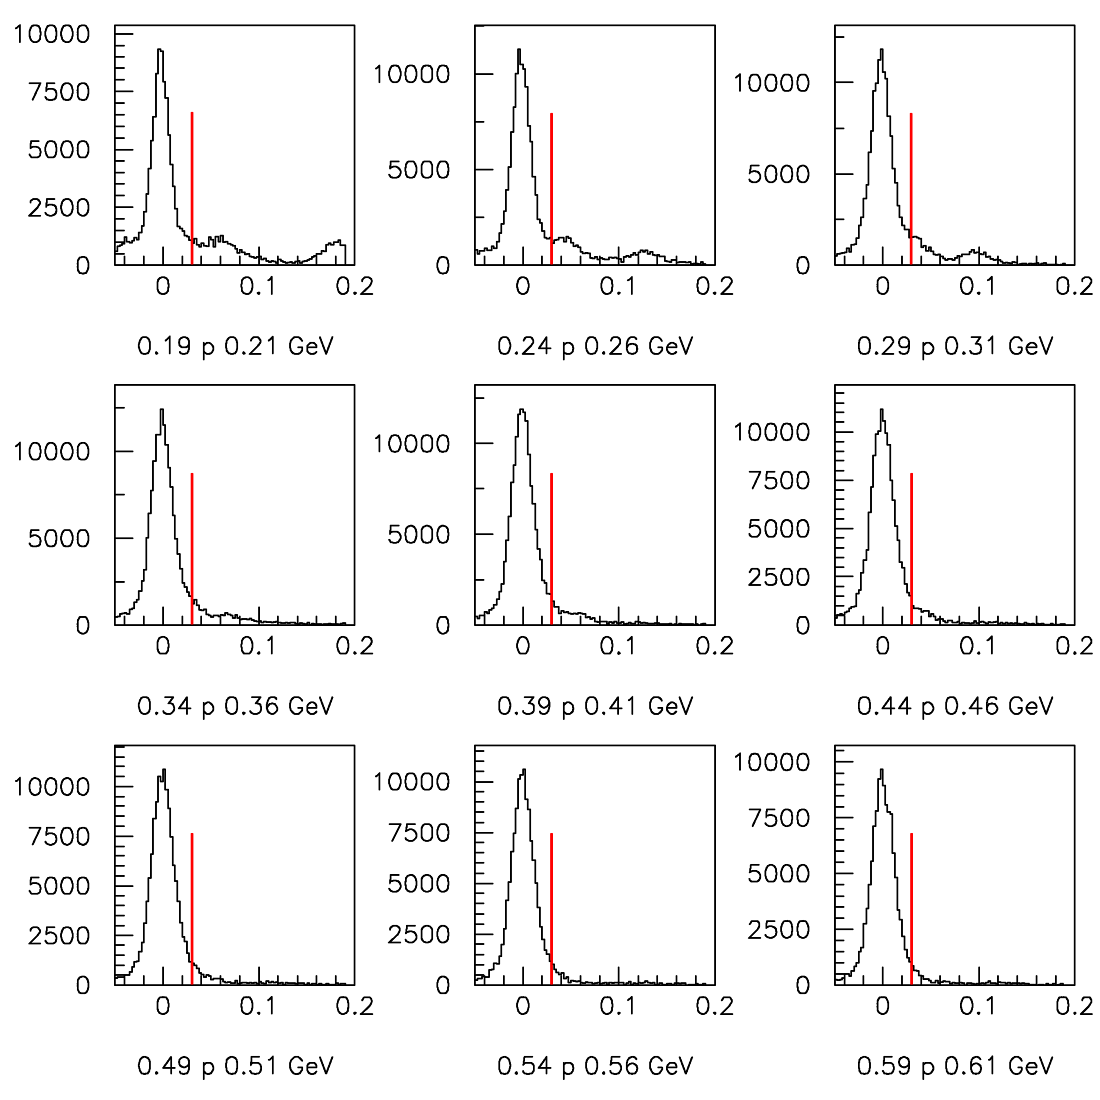
\includegraphics[width=8cm] {answer-fig/TofProfile1.png} 
\caption {$\Delta \beta$ of positively charged particles for low momentum slices 
(GeV/c). The red lines shows the applied cuts to select positive pions. The bumps on the right
correspond to muon and electron masses.}
\label{TOF-1}
\end{figure}

\begin{figure}[tbp]
\centering
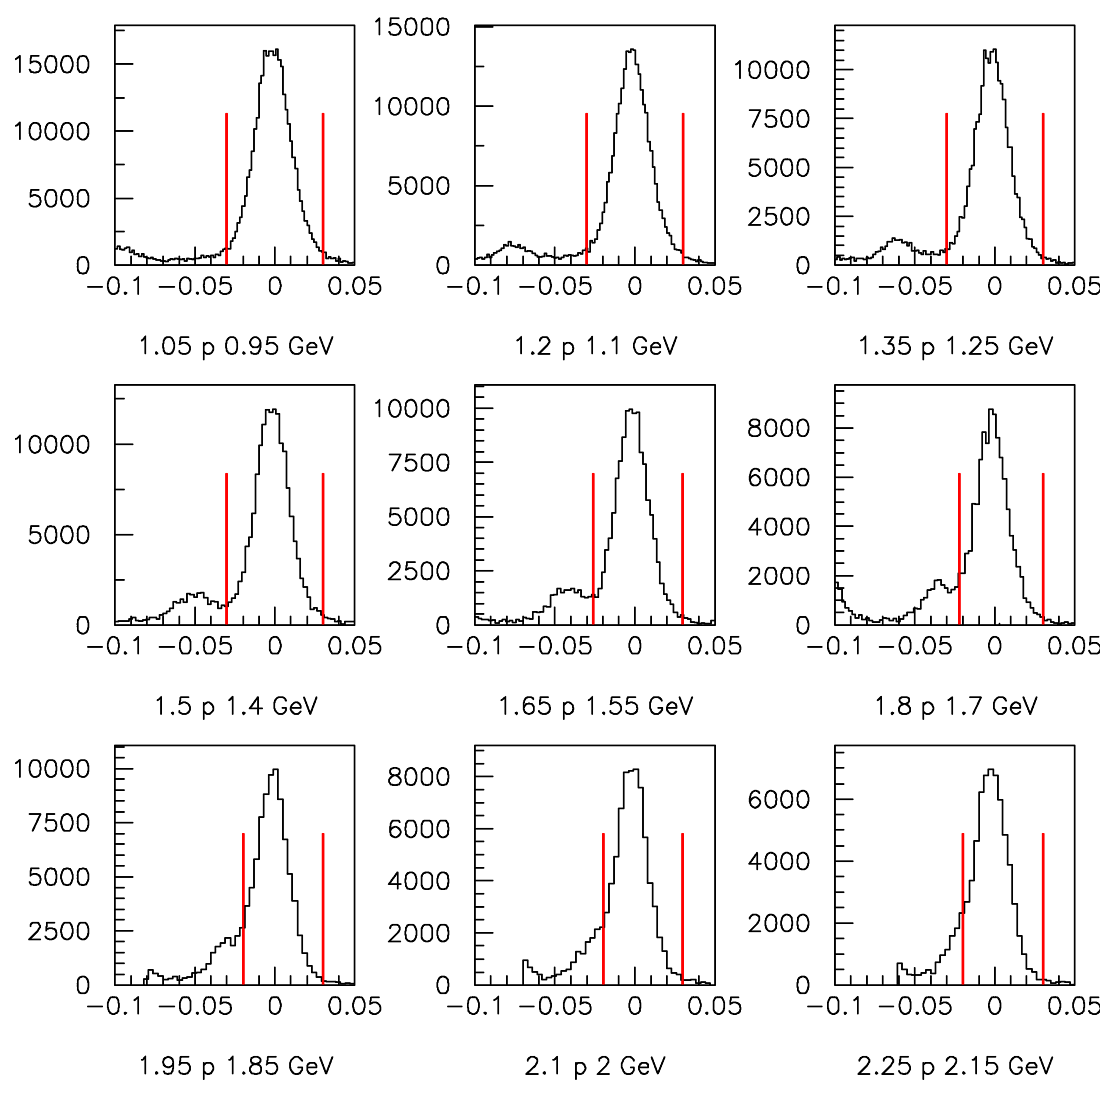
\includegraphics[width=8cm] {answer-fig/TofProfile2.png} 
\caption {$\Delta \beta$ of positively charged particles for medium momentum slices 
(GeV/c). The red lines shows the applied cuts to select positive pions. The bump on the left
correspond to the kaon mass.}
\label{TOF-2}
\end{figure}

\begin{figure}[tbp]
\centering
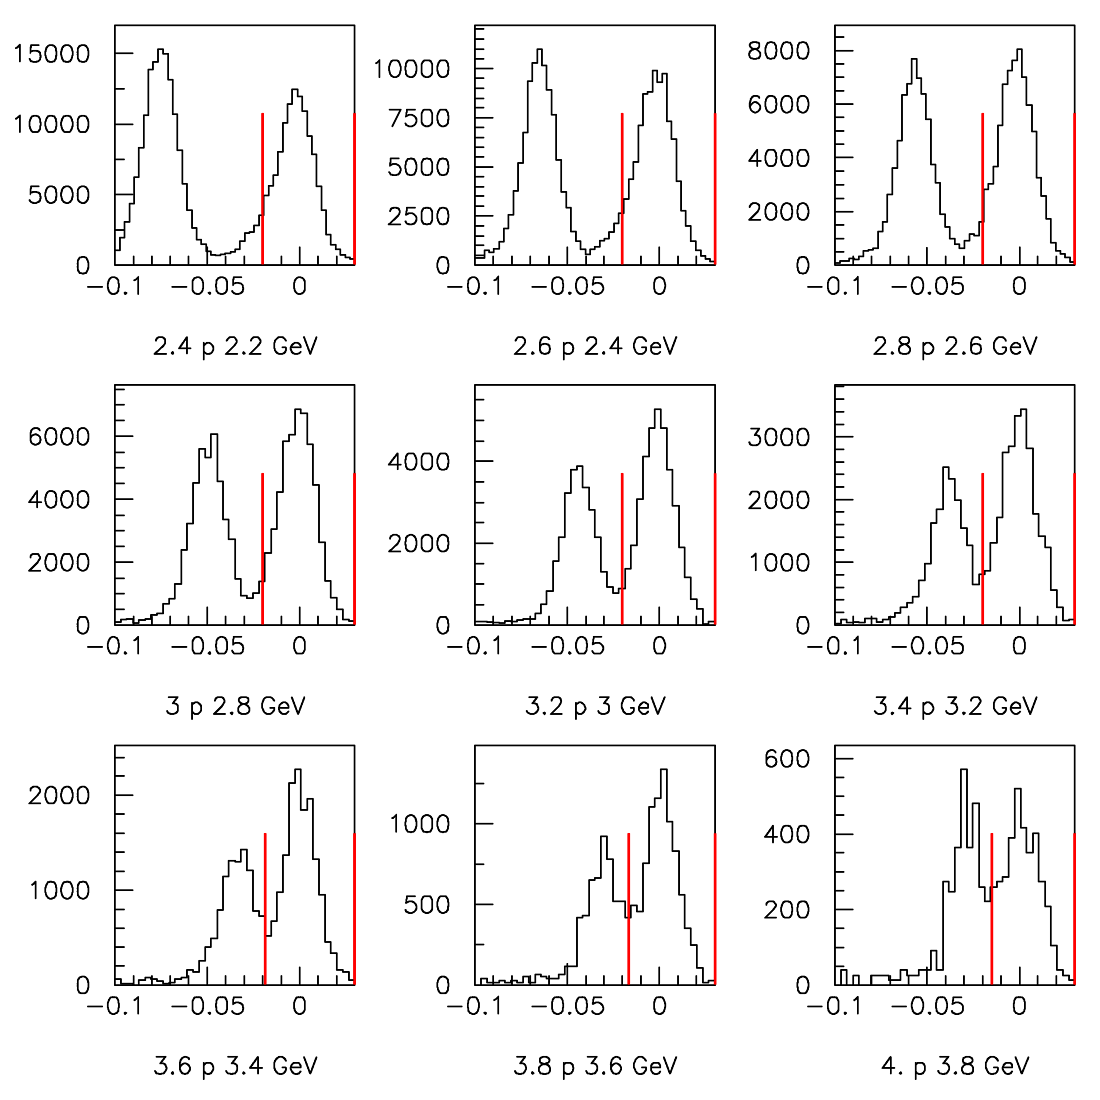
\includegraphics[width=8cm] {answer-fig/TofProfile3.png} 
\caption {$\Delta \beta$ of positively charged particles for high momentum slices 
(GeV/c). The red lines shows the applied cuts to select positive pions. The bump on the left
correspond to the proton mass.}
\label{TOF-3}
\end{figure}

5.
P16 - You state that the target position could vary from run to run, but “did not happen too 
often”.  Can you quantify this?  

{\it We show in figures \ref{VertexSolid} and \ref{VertexLiquid} the evolution 
of the position of the targets with run number. The data where the aluminum
target is off by 1 cm has been excluded from the analysis. Other variations
appear to be of a mm or less, while the gap between the solid and liquid target
is about 5 cm. They should therefore have negligible contribution to the 
error on acceptance corrections in regard to the error budget already associated
to the procedure. (This paragraph and figures are added to the note)}\\

\begin{figure}[tbp]
\centering
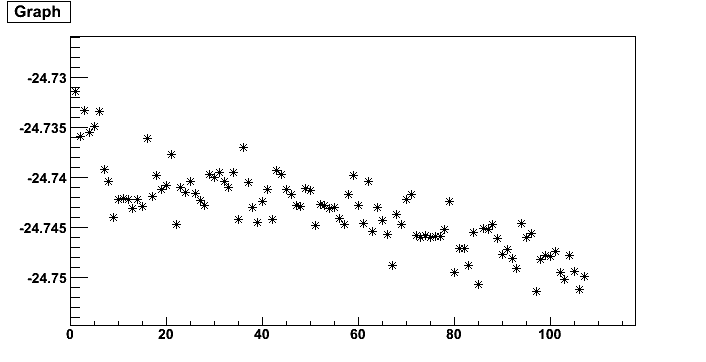
\includegraphics[width=7.5cm] {answer-fig/VertexC.png} 
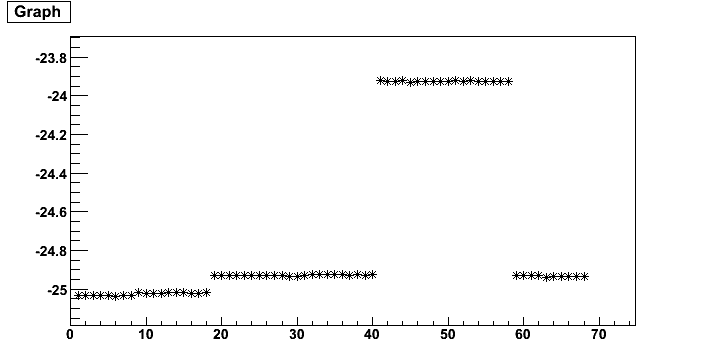
\includegraphics[width=7.5cm] {answer-fig/VertexAl.png} 
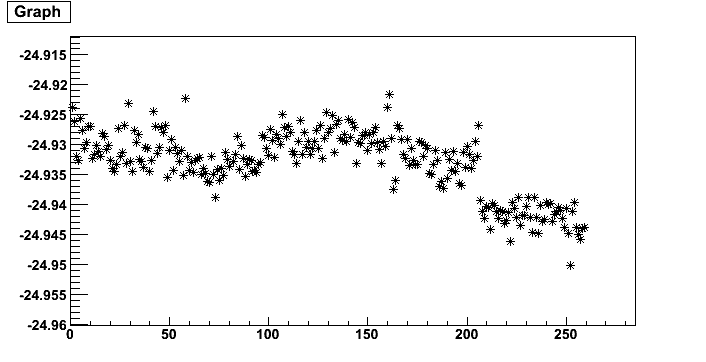
\includegraphics[width=7.5cm] {answer-fig/VertexFe.png} 
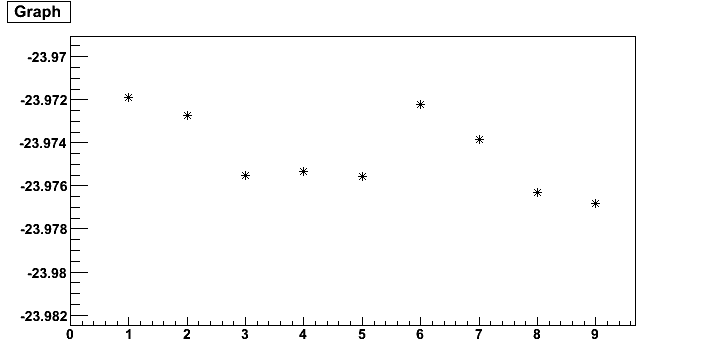
\includegraphics[width=7.5cm] {answer-fig/VertexSn.png} 
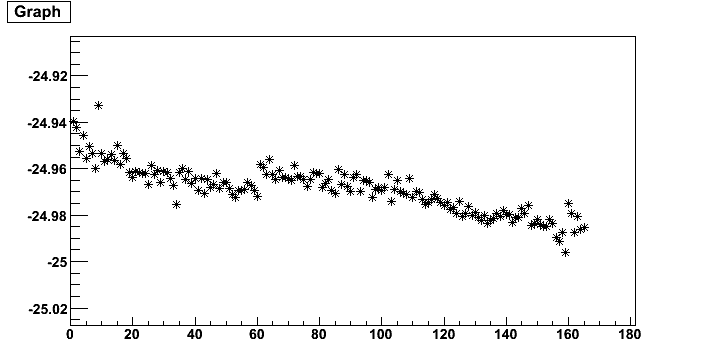
\includegraphics[width=7.5cm] {answer-fig/VertexPb.png} 
\caption {Vertex origin along $z$ (in cm) of electrons as a function of run 
number for the different solid targets.}
\label{VertexSolid}
\end{figure}

\begin{figure}[tbp]
\centering
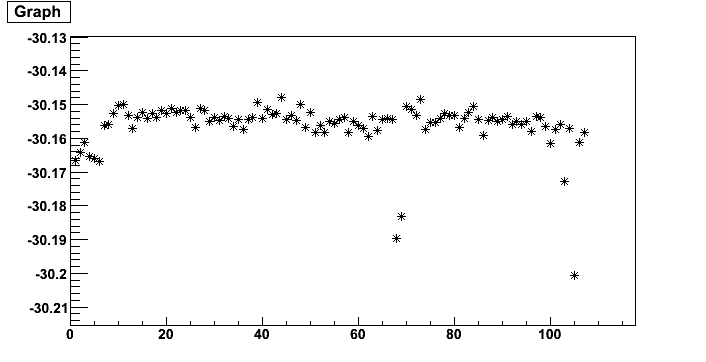
\includegraphics[width=7.5cm] {answer-fig/VertexDeutC.png} 
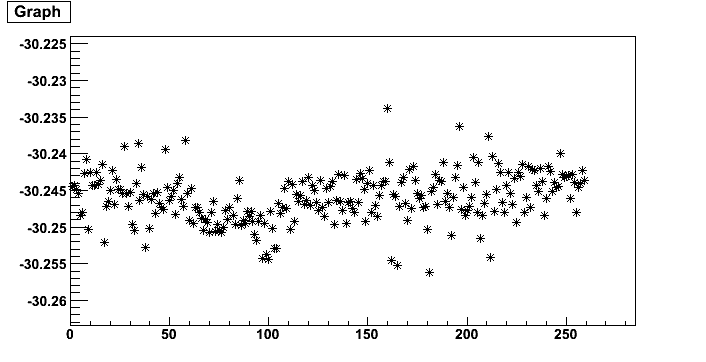
\includegraphics[width=7.5cm] {answer-fig/VertexDeutFe.png} 
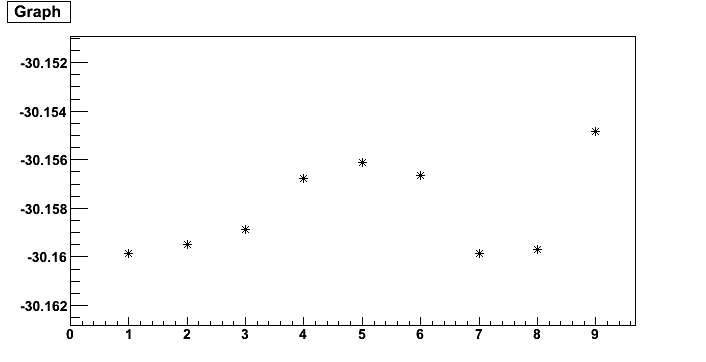
\includegraphics[width=7.5cm] {answer-fig/VertexDeutSn.png} 
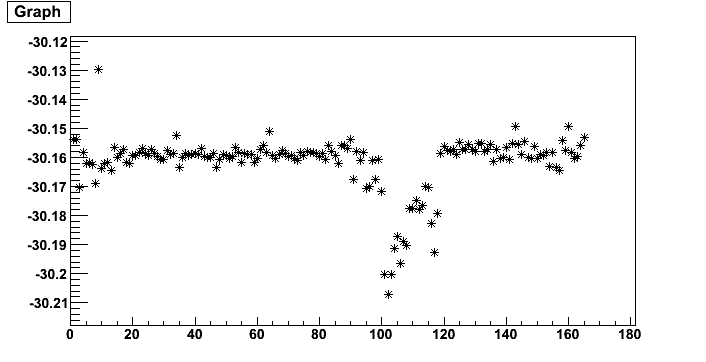
\includegraphics[width=7.5cm] {answer-fig/VertexDeutPb.png} 
\caption {Vertex origin along $z$ (in cm) of electrons as a function of run 
number for the deuterium target in different solid targets configurations.}
\label{VertexLiquid}
\end{figure}

6.
P17, Fig 12 - what solid target is shown?  Are the shifts the same for electrons and pions?

{\it Sadly, this cannot be checked, the kumac used for this figure specify a file name that
do not exist anymore (codes and files have been moved at some point and non essential files
have been removed in the process). It is always possible to reproduce the figure with a root 
routine if the reviewer feel it is necessary to know the specific run used. 

We provide here figure \ref{VertexEl} to better illustrate the result and figure 
\ref{VertexPip} to show that the pions behave similarly.}\\

\begin{figure}[tbp]
\centering
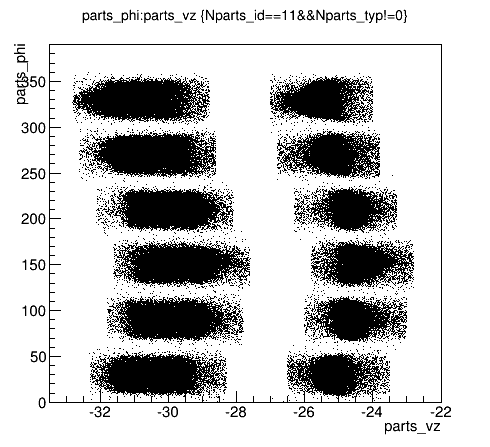
\includegraphics[width=7.5cm] {answer-fig/VertexElFe.png} 
\caption {Vertex origin along $z$ (in cm) of electrons as a function of $\phi$ 
for an iron run.}
\label{VertexEl}
\end{figure}

\begin{figure}[tbp]
\centering
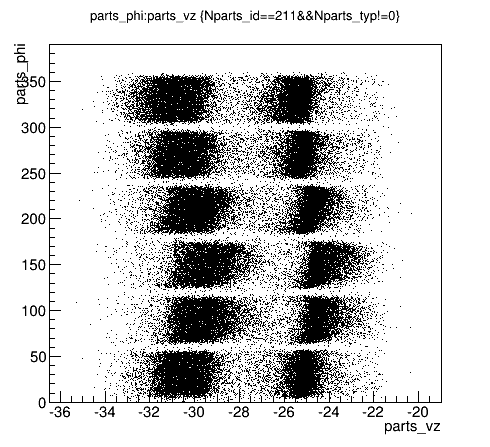
\includegraphics[width=7.5cm] {answer-fig/VertexPipFe.png} 
\caption {Vertex origin along $z$ (in cm) of positive pions as a function of $\phi$ 
for an iron run.}
\label{VertexPip}
\end{figure}

7.
P18, Start of section 2.2.5 - I’m not sure I understand the logic in this.  If you have a drift 
chamber problem, it will be manifest in both the solid and liquid target data and the ratio of 
these should be relatively stable.  Why do you not determine run quality by looking at the 
event rate per coulomb of beam current?  For this quantity, a change in the detector 
operation will show up.

{\it You are right, the motivation for this cut is not stated properly. We are looking 
at the ratio because it would affect our result, while ignoring issues that would not
affect our observable. It is important to note that the initial run list was already
cleaned from known detector failures. (The text is corrected in the note.) }


8.
P19, FIg. 14- Hard to tell how much data was discarded. Maybe give a table of means and 
sigmas for each target or show the cuts on the figure are horizontal lines.

{\it The quantity of data removed is difficult to assess, since the problematic runs were
not passed through the final analysis. We were unable to recover the orginal values of the
fits for these specific figures and we 
lack the problematic run which have been deleted. At this stage, it would be rather time
consuming to recover the raw data and update all the softwares to run on the new machines, so 
we did not produce this figure. If the reviewer think it is necessary to update this 
figure and provide more information about the discarded data let us know, it is time 
consuming but of course possible.}

9.
P19 - If you use "c" constant in dimensions of Q2, then use it for W as well.

{\it Corrected.} \\

10.
P19, Sec. 2.3 - Show plots of Q$^2$, W and y with the cuts.

{\it Figures \ref{DISKine} illustrates the request and have been added to the note.} \\

\begin{figure}[tbp]
\centering
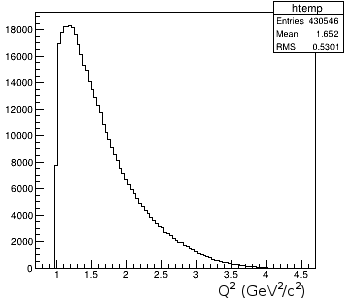
\includegraphics[width=5cm] {answer-fig/DIS-Q2.png} 
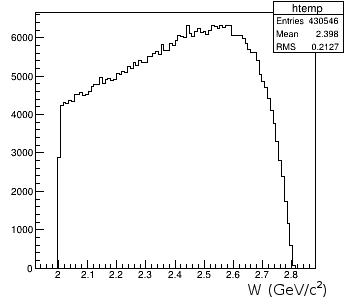
\includegraphics[width=5cm] {answer-fig/DIS-w.png} 
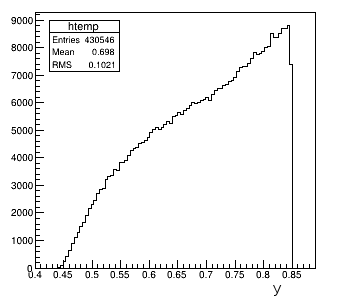
\includegraphics[width=5cm] {answer-fig/DIS-y.png} 
\caption {Inclusive distributions after DIS selection cuts for a sample of the iron
data.}
\label{DISKine}
\end{figure}


11.
P19, eq. 7 - Is it really just the sum of weights or are they the counts multiplied by the 
weights?

{\it They are indeed the counts multiplied by the weights.
The sum indicated runs over all the recorded events, it is not associated to the weight
bins or anything like that. We adapted the language in the note to make it clearer.} \\


12.
P23, I’d be very worried about the MC modeling acceptance on falling edges like that at the 
right of the top right plot.

{\it It is indeed a problematic issue, linked to the abscence of radiative effects in the 
simulation. At the time that it was generated, no better simulation was available. This
discrepency in $\nu$ motivates to also use it for the binning of the acceptance. This way,
it limits the impact of this difference.} \\


13.
P25, I find this discussion quite confusing.   At top you talk about two binnings.  It’s not just 
binning that is changing, right?  You are using different variables.  Then you talk about the 
extracted weight, but that weight is defined with only one of those sets of variables.  You 
also do it for the other set?  Then you an arbitrary weight cut to take care of the problems 
listed in the middle of the page?  Why not just increase the size of the bins in regions where 
you have too few events or large bin migration?  I don’t see how the procedure you use 
does not lead to holes in your data somehow.  And I don’t really understand what you are 
doing with the second weighting factor.  How is this not doing a double correction for 
acceptance, i.e., a double counting?  This whole section needs to be reworked.  I am fairly 
certain that I don’t really understand what you are doing but it leaves me worried that 
something is amiss.  Anyway, that’s not where you want readers to be.  

{ \it The section has been reworked to clarify what we are doing. Few points you raised 
are also answered here:

The first set of variables is the one used for the acceptance correction presented in the results,
while the second set is only used to evaluate the systematic errors associated with the correction. In the 
note, the formulas are generally given only for the first set for simplicity.

The motivation for using such a strange cut based on the product of different unrelated
values is actually directly linked to the problem of inbent 
particles being directed towards the beam pipe. The $\pi^-$ acceptance drops very 
strongly at low $p_\perp^2$ leading to very high weights, however there is no problem of 
bin migration
or low statistics because the generated yield is very high in this region. We found that 
the best way
to keep these bins while discarding bins where the size of the weight is less problematic 
but with issues concerning bin migration and statistics was to apply this type of cut.

In term of method, the two
step acceptance correction is hopefully going to be clearer. It is the same as the method used 
in the previous L. El Fassi et al. analysis note of eg2 data. The second step of the procedure is
specifically used to take care of the bins that are removed by the cut on weights. You 
can see in the formula that the weights
of the previously calculated acceptance are used in this second step, ensuring that we do not
double correct the data.

The size of the bins is not constant and is indeed increased in region with small event yield.
However, the multi dimensional binning cannot be fully adapted in a general maner. On this
topic we added tables in the note indicating the bin limits that we used.} \\

14.
P26, bottom, if you have regions with very low acceptance, should they be cut out?

{\it In the case of the $\Delta P_\perp^2$, we need to measure an average of the
transverse momentum distribution. Completely cutting a part of the distribution
would indeed solve the acceptance problems for $\pi^-$ but would make the $\langle p_\perp^2 \rangle$
measurement meaningless. We therefore have to live with it and do our best to
reconstruct the whole distribution even if it means having larger error bars.} \\


15.
P26 - "consistent with HERMES results" - could you add HERMES points to the plot with 
your data points to show what you mean as consistent?

{\it This sentence states that similarly to HERMES, we find that both charged pions have similar
transverse momentum. This can be seen in the Figure 4 of the note where we show the result from 
HERMES. We did not want to mislead the reader into any claim about compatibility between 
HERMES and CLAS data here, so we reworded the sentence. We want to point out that such claim 
would be highly model dependent since it is expected that the effect varies with energy. } \\


16.
P27 fig.22-
 It's unclear to which point the error bar is associated. I think the common 
practice is to slightly shift markers horizontally.

{\it Sorry, we overlooked this for these intermediary plots.} \\

17.
P27, Fig. 22 - the right column of plots is not the same as those in Fig. 15.  Why change the 
variables?

{\it Sorry, it is a mistake on our part, there is no reason.} \\

18.
P28 - What is Coulolmb Correction applied to? Momentum of charged particles? Could you 
plot effect of this correction on particles? Is it really big enough to be visible within our 
resolutions ?

{\it The Coulomb correction is applied to incoming and outgoing electrons as well as
produced charged pions. Indeed the effect is small in most of the phase space, but 
by slightly shifting the $z$ distribution it slightly changes the normalization. A
point to point effect is also visible for low $z$ pions. Note that in general, there
is also a focussing factor in Coulomb corrections, but they happen to cancel out in
our specific observables.} \\


19.
P30 - 
fig.24 is missing X axis label. You also may consider 2D histogram for better display.

{\it This figure is replaced by others in the new radiative correction section.} \\


20.
P31 - I don’t understand the isospin correction.  It does smooth out the data in Fig. 27; 
however, I am missing the physics motivation.  Why does it matter if the quark came from a 
proton or a neutron?  I think you just clarify the explanation.

{\it This correction is here to take care of the u/d quark imbalance in heavier nuclei.
Indeed the multiplicity of positive pions on neutrons is significantly smaller than on protons and that
should not be mistaken with absorbtion in the nuclear medium. We clarified the text in the
note.} \\


21.
P33, Sec. 2.5.1 - list the negligible effects.

{\it The sentence has been revised to list all effects tested.} \\

22.
P34, Fig. 28 - why is the resolution poorer than in Fig. 12?

{\it Resolution is the same, it looks wider because, on this figure, we show the integrated 
result over the 6 sectors, which are slightly shifted between each other.} \\


23.
P34, why do you have a 1\% normalization error in all the multiplicity ratios when you say just 
above that for this particular sample with two particles in the final state the events in the test 
regions dropped to 0.01?  Doesn’t that mean the target contamination normalization error is 
smaller than 1\%?

{\it Multiplicity ratios are a double ratio. The claim is that the semi-inclusive part 
is not affected, but the inclusive electron ratio is affected. This is included
as a normalisation error. We revisited the paragraph to make this point clearer.} \\


24.
P34, with this technique of comparing results using the two different sets of variables (you 
call it two binnings, but I think that is sort of misleading), you are using the same events.  
Does this not mean you have a statistical contribution to this systematic error?  You say you 
noticed larger systematic errors for the pi- events due to lower acceptance and bigger 
weights.  Might it also be lower statistics and so you have statistical fluctuations contributing 
to the systematic error?  If so, you are sort of double-counting the statistical error and 
inflating the systematic error more than it should be.  

{\it This is an interesting question and we might have overlooked this problem. Looking into the
issue we noticed an error in our function calculating the statistical errors. This change 
would modify our initial statement. Altogether, after reviewing the question, we believe that 
because the different acceptance are calculated from the same simulated data and applied to 
the same experimental data, our systematic error calculation should not include the effect 
of statistical errors. In conclusion, we removed the previous statement and now fully include 
the systematic errors for the transverse momentum broadening.} \\

25.
P35 - It would clarify the discussion with a summary or table of the point-to-point systematic 
errors.

{\it The point-to-point errors include only contributions from the particle 
identifications and acceptance effects. It is also different for every bin, so
we did not think a table would be useful to summarize only two contributions.} \\

26.
P35 -
 add plots with systematic uncertainty bands on it to demonstrate bin-by-bin values.

{\it We add this on the figures intended to be published.} \\


27.
P35, end of top paragraph, you say you don’t include the acceptance systematic, but it looks 
to me like it is included in Table 8?  What am I missing?

{\it We decided to keep the normalization error, not the point to point. This was not
said clearly in the text, it is now changed as mentioned above.} \\


28.
P36, top paragraph, “that a factorization holds” means what??  Should explain.  

{\it This sentence has been reformulated with an additional reference.} \\


29.
P36 top of section 3.1.1, 5\% versus 5\% looks more like 1 sigma rather than the 1.5 sigma 
you say in the text.

{\it The reson we quote 1.5, is that one need to move $\pi^+$ one sigma down and $\pi^-$ one
sigma up. So for the overall normal deviation (sigma) we quadratically sum them,
leading to 1.5, you think it should say 2?} \\

30.
P36, second paragraph of section 3.1.1, “... might be modified if the production time occurs 
inside the nucleus.”  I think I know what you mean but the language makes no sense.  You 
mean if the formation takes place inside the nucleus, right?

{\it This langage refers to figure 1, where we define a production time and a 
formation time. We rephrased for more clarity.}\\

31.
P42, top, “... that is seen in our result.”  Where do I see what you are discussing in the top 
two lines of this page.  I could not find whatever it is.  What should I be looking at?

{\it The phrasing was incorrect, hopefully the new version is better. We will work with 
the authors of the models to add some projections to our figures. This should eventually
make all these physics comments much clearer.} \\

\section{Typographical Corrections}

Abstract L2, “... non-perturbative; therefore, only...”

P3, para 2:  “... models, including ones relevant for RHIC, because the size of the cold nuclei 
used in the JLab experiments is stable and known.”

P4, L1, “... the study of pion production over ...”

P4, L3, “... section 1.3, we provide a...”

P5, para 3, L3, “This kind of model is suitable...”

P6, L4, “... a suppression of hadron production ...and it can even reverse sign and increase at 
very low z.”

P6, bottom paragraph, line 3, “... excess in delta(pt)\^2.  It is notable that ... behavior in models 
... models do not yet treat baryon hadronization.”

P9, L6, “filled with liquid deuterium”

P9, para2, end of para, “... and detector properties cancel in the nuclear ratio.”

P10, L2, okay for a technical note but here the sentence should be rephrased to something like 
“For pions, we require a signal in the drift chambers (DC) and scintillator counters (SC) in 
addition to the successful reconstruction of the time-based tracking.”

P10, L10, “The derivation of these quantities is presented in section 2.3, while a list of 
corrections  is summarized in section 2.4.  The systematic uncertainty budget is detailed in 
section 2.5, and ...”

P10, just below equation 3, “ ... and the parameter b varies with momentum, as ...”

P13, L1 of section 2.2.2, sentence makes no sense as written. Do you mean something like, 
“Negatively charged pion candidates must not pass the electron selection criteria.”

P15, L2 of section 2.2.3 “... (see figure 11) due to a significant...”

P15 bottom, “These cuts minimize the kaon...”

P18, 6 lines from the bottom - “As Figure 14 ...”

P20, L1 of section 2.3.2 “... in figure 15 a few ...”

P21, L2, “... processed by CLAS software (GSIM, GPP and user\_ana) [what do these mean to a 
non-CLAS reader? supply references] to simulate the detector and the reconstruction process in 
a fashion similar to that done with the experimental data.”
Start of next paragraph, “The simulated data are processed like the experimental data by 
applying ...”  “ ... quite well the detector response, yet ...” \\

{\it Not sure what reference we should add here. The analysis note is not only a technical document
it is also an internal document.} \\

P22, bottom, “... space of our two-particle final state.  However, to evaluate the systematic 
errors associated with ...”

P33, 2 lines from bottom, “re-scattering on detector material”

P35, top of section 2.5.4, “... contributions from particle misidentification and acceptance ... 
effects, target misidentification and the isospin ...”

P36, second paragraph of section 3.1.1 -
 change conciliate to reconcile

P38, Para 3, L2, change signification to significance

P38, bottom, “However, our results (figure 32(left)) show no dependence besides ... and what is 
left will be washed ...”

P41, first paragraph, what does HERMES say about Q2 dependence?  Line 4, “... in figure 34, 
does not indicate ...” \\

{\it HERMES do see an increase which is not statistically significant 
(see figures 2 and 3 of the note).} \\

P41, bottom paragraph, “... wide A coverage gives a outright indication ... found to be much 
smaller than that seen by HERMES [15], which ....from BDMPS [29] correlate pt\^2 with the 
nuclear radius.”

P42, top paragraph, last line, “colored parton does not interact with the whole nucleus which 
limits the nuclear effect.”

P42 second paragraph, L2, “they predict a rise of delta pt\^2 with Q\^2”
Same paragraph, L4, “... 38) gives a similar result.” \\

{\it Sorry for the clumsy English in some parts. We have implemented all the 
suggested changes and some more. This issue should now be solved.} \\

\end{document}
